% =============================================================================
% Le Petit Guide du Stacker — BullionRadar.fr
% Édition 2026
% =============================================================================
\documentclass[14pt,a4paper]{extarticle}

% --- Encodage et langue (xelatex) ---
\usepackage{fontspec}
\usepackage[french]{babel}
\usepackage{textcomp}
\newcommand{\permil}{‰}

% --- Mise en page ---
\usepackage[margin=2.5cm,headheight=22pt]{geometry}
\usepackage{setspace}
\onehalfspacing
\usepackage{parskip}
\usepackage{enumitem}

% --- Graphiques et couleurs ---
\usepackage{graphicx}
\usepackage[dvipsnames]{xcolor}
\usepackage{tikz}
\usetikzlibrary{calc,positioning}

% --- Tableaux ---
\usepackage{booktabs}
\usepackage{array}
\usepackage{colortbl}

% --- En-tête et pied de page ---
\usepackage{fancyhdr}
\pagestyle{fancy}
\fancyhf{}
\fancyhead[L]{\small\textbf{\textcolor{gold}{BullionRadar.fr}}}
\fancyhead[R]{\small\textit{\textcolor{gold}{Le Petit Guide du Stacker}}}
\fancyfoot[C]{\thepage}
\renewcommand{\headrulewidth}{0.5pt}
\renewcommand{\headrule}{\hbox to\headwidth{\color{gold}\leaders\hrule height \headrulewidth\hfill}}

% --- Liens ---
\usepackage[colorlinks=true,linkcolor=gold,urlcolor=gold]{hyperref}

% --- Couleurs personnalisées ---
\definecolor{gold}{HTML}{BE943C}
\definecolor{darkbg}{HTML}{1A1A1A}
\definecolor{darkcard}{HTML}{2A2A2A}
\definecolor{lightgold}{HTML}{D4A84B}
\definecolor{textgold}{HTML}{BE943C}

% --- Titres en couleur or ---
\usepackage{titlesec}
\titleformat{\section}{\LARGE\bfseries\color{gold}}{}{0em}{}
\titleformat{\subsection}{\Large\bfseries}{}{0em}{}
\titleformat{\subsubsection}{\large\bfseries}{}{0em}{}

% --- Séparateur décoratif ---
\newcommand{\goldsep}{%
  \begin{center}
    \textcolor{gold}{\rule{6cm}{0.4pt}}
  \end{center}
}

% =============================================================================
\begin{document}

% =============================================================================
% PAGE DE COUVERTURE
% =============================================================================
\begin{titlepage}
\centering
\vspace*{2cm}

{\Large Le Petit Guide du Stacker}\\[0.5cm]
{\normalsize BullionRadar.fr}\\[0.2cm]
{\normalsize 2026}

\vspace{2cm}

% Image bonhomme coffre-fort
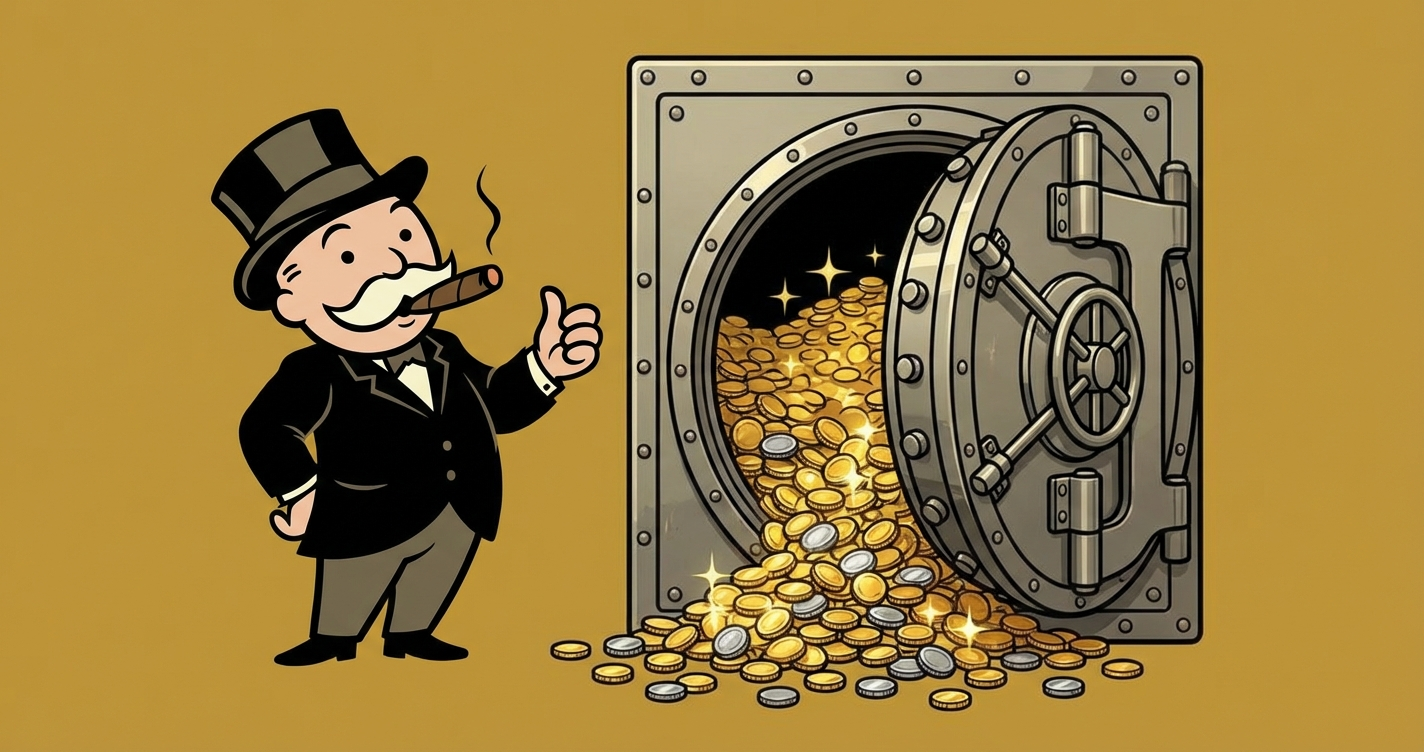
\includegraphics[width=5cm]{../../public/images/bonhomme-coffre-fort.jpeg}

\vspace{1.5cm}

{\Huge\bfseries\textcolor{gold}{Le Petit Guide du Stacker}}

\vspace{0.8cm}

{\large\textcolor{gold!70}{Tout ce qu'il faut savoir pour stacker\\de l'or et de l'argent physique en France}}

\vspace{2cm}

{\large\textbf{BullionRadar.fr}}\\[0.3cm]
{\normalsize Le comparateur indépendant de pièces d'or et d'argent}

\vspace{1.5cm}

{\normalsize Édition 2026 --- Guide gratuit}

\end{titlepage}

% Table des matières
{
\setlength{\parskip}{6pt}
\renewcommand{\baselinestretch}{1.8}\normalsize
\tableofcontents
}
\newpage

% =============================================================================
% INTRODUCTION
% =============================================================================
\section*{Introduction}
\addcontentsline{toc}{section}{Introduction}

\begin{center}
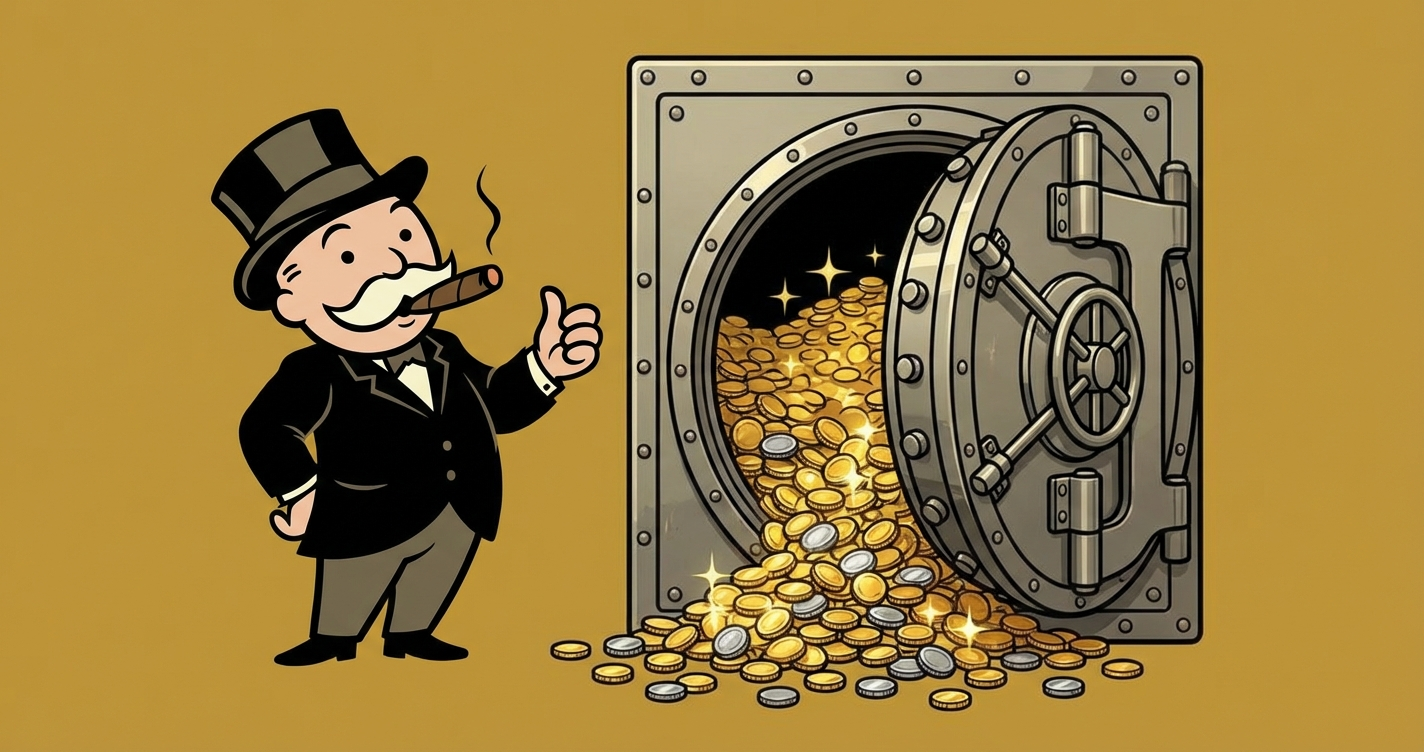
\includegraphics[width=3.5cm]{../../public/images/bonhomme-flipping-coin.jpeg}
\end{center}

Bienvenue dans \textbf{Le Petit Guide du Stacker}. Ce guide a pour objectif de vous accompagner dans vos premiers pas dans l'accumulation de pièces d'or et d'argent physiques.

\textbf{Stacker} (de l'anglais \textit{to stack}, empiler) : terme utilisé dans la communauté des métaux précieux pour désigner un investisseur qui accumule méthodiquement de l'or et de l'argent physiques sur le long terme.

L'or et l'argent sont des \textbf{valeurs refuges depuis des millénaires}. Aujourd'hui, stacker des \textit{bullion coins} reste l'un des moyens les plus accessibles de diversifier son patrimoine et de se protéger contre l'inflation.

\begin{quote}
\textit{«~L'or est la monnaie des rois, l'argent est la monnaie des gentilshommes.~»}
\end{quote}

\newpage

% =============================================================================
% CHAPITRE 1 : POURQUOI STACKER
% =============================================================================
\section{Chapitre 1 : Pourquoi stacker de l'or et de l'argent~?}

\subsection{Le debasement trade}

Le 15 août 1971, le président Nixon met fin unilatéralement aux accords de Bretton Woods~: le dollar n'est plus convertible en or. Ce jour-là, toutes les monnaies du monde deviennent des monnaies \textit{fiat} (du latin \textit{fiat} --- «~qu'il en soit ainsi~»), c'est-à-dire des monnaies \textbf{sans aucune contrepartie physique}. Leur valeur ne repose plus que sur la confiance dans les gouvernements qui les émettent.

\textbf{Qu'est-ce que cela signifie concrètement~?} Depuis 1971, les banques centrales peuvent imprimer autant de billets qu'elles le souhaitent, sans contrainte. Et c'est exactement ce qu'elles font~: la masse monétaire M2 aux États-Unis est passée de 600 milliards de dollars en 1971 à plus de \textbf{21\,000 milliards en 2026} --- une multiplication par 35. La BCE n'est pas en reste~: entre 2015 et 2023, elle a injecté plus de \textbf{5\,000 milliards d'euros} dans le système via ses programmes de rachat d'actifs (\textit{Quantitative Easing}).

Chaque billet imprimé sans contrepartie de richesse réelle \textbf{dilue la valeur de tous les billets déjà en circulation}. C'est la définition même du \textit{debasement} --- la dévaluation progressive et silencieuse de votre épargne.

\textbf{Les chiffres parlent d'eux-mêmes~:}
\begin{itemize}
  \item Depuis 1971, le dollar a perdu \textbf{plus de 98\% de son pouvoir d'achat} mesuré en or
  \item L'euro a perdu environ \textbf{85\% de sa valeur} face à l'or depuis sa création en 1999
  \item En 2000, une once d'or valait $\sim$300\,€. En 2026, elle dépasse les 5\,000\,€
  \item 100\,€ placés sur un livret A en 2000 valent environ 65\,€ en pouvoir d'achat réel aujourd'hui
\end{itemize}

\textbf{La spirale de la dette~:} les pays occidentaux sont endettés à des niveaux sans précédent en temps de paix. La France dépasse les \textbf{110\% du PIB} de dette publique (plus de 3\,200 milliards d'euros), les États-Unis les \textbf{130\%} (36\,000 milliards de dollars), le Japon les \textbf{260\%}. Ces dettes ne seront jamais remboursées au sens classique du terme. La seule issue politiquement acceptable est de les \textbf{diluer par l'inflation et la création monétaire} --- c'est-à-dire en imprimant encore plus de billets, ce qui accélère encore la perte de valeur des monnaies fiat.

C'est un cercle vicieux~: plus de dette $\rightarrow$ plus d'impression monétaire $\rightarrow$ plus d'inflation $\rightarrow$ plus de dette pour financer les déficits\ldots

Le \textit{debasement trade} consiste à se positionner sur des actifs réels (or, argent physique) pour se protéger de cette érosion monétaire structurelle. Ce n'est pas de la spéculation --- c'est de la \textbf{préservation de patrimoine}. Quand les monnaies fiat perdent de la valeur, l'or et l'argent en gagnent mécaniquement, car leur quantité est limitée par la nature~: on ne peut pas «~imprimer~» de l'or.

\subsection{L'inflation rampante}

Les chiffres officiels d'inflation (IPC) sous-estiment systématiquement la perte de pouvoir d'achat réelle. Entre la \textit{shrinkflation} (réduction des quantités à prix constant), l'\textit{hédonique} (ajustements qualité qui masquent les hausses), et les changements méthodologiques, l'inflation ressentie est souvent le double de l'inflation officielle.

\textbf{L'or comme couverture historique~:}
\begin{itemize}
  \item Sur les 50 dernières années, l'or a surperformé l'inflation dans \textbf{80\% des décennies}
  \item Pendant les périodes de forte inflation (années 70, 2021--2025), l'or a systématiquement accéléré
  \item L'argent, plus volatile, offre un effet de levier encore plus important en période inflationniste
\end{itemize}

\textbf{Exemple concret~:} un épargnant qui a placé 10\,000\,€ sur un Livret A en 2000 a environ 14\,000\,€ aujourd'hui. Le même montant investi en or physique vaut plus de 80\,000\,€. La différence, c'est l'inflation réelle que le Livret A n'a jamais compensée.

\subsection{Incertitude géopolitique}

Le monde entre dans une phase de \textbf{fragmentation géopolitique} sans précédent depuis la Guerre froide~:

\begin{itemize}
  \item \textbf{Guerres commerciales} : tarifs douaniers, sanctions économiques, weaponisation du dollar
  \item \textbf{Dédollarisation} : de plus en plus de pays commercent en monnaies locales (yuan, roupie, rouble)
  \item \textbf{Tensions militaires} : Ukraine, Taïwan, Moyen-Orient --- chaque escalade fait monter l'or
  \item \textbf{Sanctions financières} : le gel des réserves russes en 2022 a montré que même les obligations souveraines ne sont plus «~sûres~»
\end{itemize}

Dans ce contexte, l'or physique est le seul actif qui n'a \textbf{aucun risque de contrepartie}. Pas de banque qui peut faire faillite, pas de gouvernement qui peut le geler, pas de serveur qui peut tomber en panne.

\subsection{Ce que font les banques centrales des BRICS}

Si vous voulez savoir où va l'or, regardez ce que font ceux qui impriment la monnaie.

\textbf{Achats records des banques centrales~:}
\begin{itemize}
  \item \textbf{2022--2025} : les banques centrales ont acheté plus de \textbf{1\,000 tonnes d'or par an}, un record historique
  \item \textbf{Chine (PBoC)} : achats officiels continus depuis 2022, mais les achats réels (via des intermédiaires) sont estimés 2 à 3 fois supérieurs
  \item \textbf{Russie} : a remplacé ses réserves en dollars par de l'or --- aujourd'hui plus de 2\,300 tonnes
  \item \textbf{Inde (RBI)} : achats réguliers, rapatriement d'or stocké à Londres
  \item \textbf{Turquie, Pologne, Singapour} : tous acheteurs nets
\end{itemize}

\textbf{Le message est clair~:} les banques centrales, qui connaissent mieux que quiconque la fragilité du système monétaire, accumulent de l'or physique à un rythme sans précédent. Le stacker fait exactement la même chose, à son échelle.

\subsection{Couverture contre un crash boursier tech/AI}

Les marchés boursiers mondiaux sont aujourd'hui \textbf{dangereusement concentrés}~:

\begin{itemize}
  \item Les «~Magnificent 7~» (Apple, Microsoft, Nvidia, Amazon, Google, Meta, Tesla) représentent à eux seuls plus de \textbf{30\% du S\&P 500}
  \item Les valorisations de certaines entreprises AI intègrent des scénarios de croissance \textbf{extrêmement optimistes}
  \item Historiquement, chaque révolution technologique (chemins de fer, dotcom, etc.) a connu une phase de bulle puis de correction sévère
\end{itemize}

L'or a une \textbf{corrélation faible, voire négative}, avec les marchés actions~:
\begin{itemize}
  \item Pendant le crash dotcom (2000--2002) : actions $-$50\%, or $+$12\%
  \item Pendant la crise de 2008 : actions $-$57\%, or $+$25\% (sur 2008--2009)
  \item Pendant le COVID (mars 2020) : l'or a récupéré en quelques semaines, puis atteint de nouveaux records
\end{itemize}

Avoir 5 à 15\% de son patrimoine en métaux précieux physiques n'est pas un pari contre la tech --- c'est une \textbf{assurance} au cas où les choses tournent mal.

\subsection{La vision contrarian}

Le consensus mainstream (banques, médias financiers, conseillers patrimoniaux) a \textbf{systématiquement sous-estimé l'or} depuis 20 ans. En 2000, l'once était à 300\,€ et «~personne n'en voulait~». En 2026, elle dépasse 5\,000\,€.

\textbf{Pourquoi le consensus se trompe~:}
\begin{itemize}
  \item Les banques ne gagnent pas de commissions récurrentes sur l'or physique (contrairement aux fonds, assurances-vie, etc.)
  \item Les médias financiers vivent de la publicité des institutions financières
  \item L'or physique est «~ennuyeux~» --- pas de dividende, pas de croissance trimestrielle à annoncer
\end{itemize}

\textbf{La réalité~:} l'or a surperformé le CAC 40, le S\&P 500, et l'immobilier parisien sur les 25 dernières années. Silencieusement, sans fanfare.

Le stacker est par nature un \textbf{contrarian}. Il ne cherche pas le rendement à court terme. Il accumule patiemment un actif que les générations précédentes ont toujours considéré comme la réserve de valeur ultime.

\begin{quote}
\textit{«~Achetez quand personne n'en veut. Quand tout le monde en voudra, vous aurez déjà le vôtre.~»}
\end{quote}

\newpage

% =============================================================================
% CHAPITRE 2 : LES PIÈCES D'OR À STACKER
% =============================================================================
\section{Chapitre 2 : Les pièces d'or à stacker}

\begin{center}
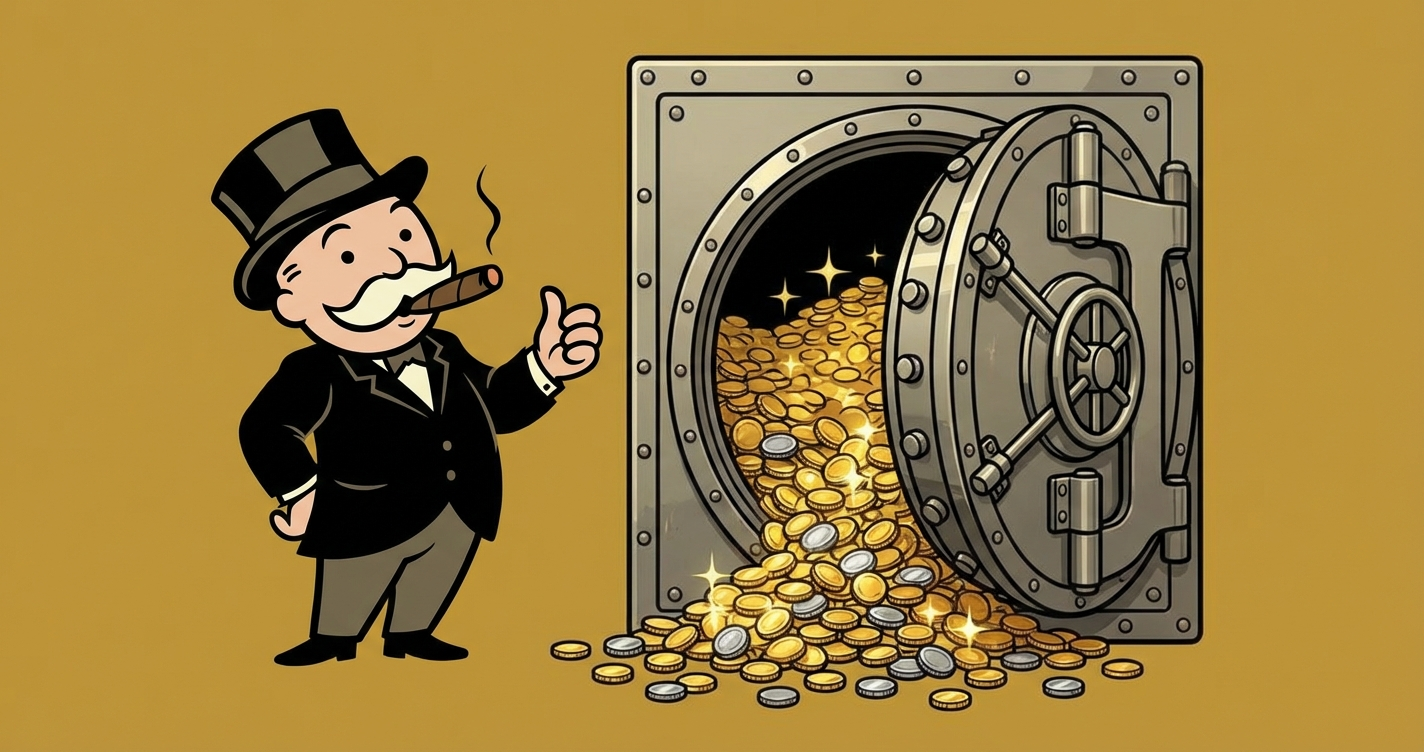
\includegraphics[width=3.5cm]{../../public/images/bonhomme-flipping-coin.jpeg}
\end{center}

L'or d'investissement est \textbf{exonéré de TVA} en France (et dans toute l'UE). Que vous achetiez un Krugerrand, une Maple Leaf ou un Napoléon, vous ne payez que le prix du métal plus la prime du dealer. C'est un avantage fiscal considérable par rapport à l'argent.

Voici les pièces d'or bullion incontournables, celles que tout stacker devrait connaître.

\subsection{Les pièces 1 once}

\subsubsection{1. Krugerrand (Afrique du Sud)}

\textbf{South African Mint (Pretoria) --- 916,7\permil{} --- 33,93\,g}

\textbf{Première pièce d'investissement moderne}, lancée en 1967. Alliage 22 carats (91,67\% or, 8,33\% cuivre) qui lui donne sa couleur orangée caractéristique et une résistance supérieure aux rayures. La pièce la plus stackée au monde avec plus de 50 millions d'exemplaires.

\textit{Pourquoi la stacker~:} Liquidité absolue, reconnue partout dans le monde. Pas de valeur faciale --- sa valeur est purement celle de son contenu en or. Le standard historique du bullion.


\goldsep

\subsubsection{2. Maple Leaf (Canada)}

\textbf{Monnaie royale canadienne (Ottawa) --- 999,9\permil{} --- 31,10\,g}

La Maple Leaf a été la \textbf{première pièce bullion en or pur 999,9} au monde lors de son passage à 4 neuf en 1982. Depuis 2013, elle intègre une micro-gravure laser (une petite feuille d'érable visible uniquement au microscope) et des lignes radiales comme dispositifs anti-contrefaçon parmi les plus avancés du marché.

\textit{Pourquoi la stacker~:} Pureté maximale (999,9), sécurité anti-contrefaçon de pointe, prime raisonnable. Le choix naturel du stacker qui veut de l'or le plus pur possible.


\goldsep

\subsubsection{3. American Eagle (États-Unis)}

\textbf{United States Mint --- 916,7\permil{} --- 33,93\,g}

L'Eagle est la \textbf{pièce d'or la plus vendue aux États-Unis}. Alliage 22 carats (or, argent, cuivre) qui la rend plus résistante aux manipulations. Son avers «~Walking Liberty~» est l'un des designs les plus iconiques de la numismatique mondiale. En 2021, le revers a été modernisé avec un nouveau motif d'aigle (Type 2).

\textit{Pourquoi la stacker~:} Liquidité maximale sur le marché américain et international. Seule pièce d'or éligible aux IRA (comptes retraite) américains. La référence absolue outre-Atlantique.


\goldsep

\subsubsection{4. Philharmonique (Autriche)}

\textbf{Münze Österreich (Vienne) --- 999,9\permil{} --- 31,10\,g}

Or pur 24 carats. \textbf{La pièce d'or la plus stackée en Europe.} Émise par la Monnaie d'Autriche depuis 1989, elle célèbre l'Orchestre philharmonique de Vienne. C'est la \textbf{seule pièce bullion majeure libellée en euros} (valeur faciale 100\,€), ce qui en fait le choix naturel pour les investisseurs de la zone euro.

\textit{Pourquoi la stacker~:} Aucun portrait de monarque (instruments de musique), libellée en euros, prime parmi les plus basses du marché. Le choix rationnel du stacker européen.


\goldsep

\subsubsection{5. Britannia (Royaume-Uni)}

\textbf{The Royal Mint (Llantrisant) --- 999,9\permil{} --- 31,10\,g}

Britannia, figure allégorique de la Grande-Bretagne depuis l'époque romaine, orne cette pièce émise depuis 1987. Depuis 2021, elle intègre des \textbf{technologies anti-contrefaçon parmi les plus avancées du marché}~: lignes radiales, image latente, marquage micro-textuel sur le trident. L'avers porte désormais le portrait de Charles III (2023).

\textit{Pourquoi la stacker~:} Sécurité anti-contrefaçon de pointe, prime compétitive ($\sim$6,5\%), design iconique qui évolue chaque année. Exonérée de CGT au Royaume-Uni.


\goldsep

\subsubsection{6. American Buffalo (États-Unis)}

\textbf{United States Mint --- 999,9\permil{} --- 31,10\,g}

Lancée en 2006, le Buffalo est la \textbf{première pièce d'or américaine en or pur} (999,9). Son design est inspiré du célèbre nickel Buffalo de 1913~: un Amérindien à l'avers, un bison américain au revers. Pour les stackers qui veulent de l'or américain ET de l'or pur, c'est le seul choix.

\textit{Pourquoi la stacker~:} La pureté de la Maple Leaf combinée au prestige américain. Design historique parmi les plus beaux de la numismatique US. Liquidité excellente.


\goldsep

\subsubsection{7. Kangourou (Australie)}

\textbf{The Perth Mint (Perth) --- 999,9\permil{} --- 31,10\,g}

Originellement appelée «~Gold Nugget~» (1986--1989), cette pièce a été renommée Kangourou en 1989. Sa particularité~: le \textbf{design du kangourou change chaque année}, ce qui lui donne un attrait à la fois bullion et collectionneur. La Perth Mint offre une garantie de rachat à vie.

\textit{Pourquoi la stacker~:} Pureté maximale (999,9), design annuel attractif, garantie Perth Mint. Excellente alternative pour diversifier son stack géographiquement.


\goldsep

\subsubsection{8. Libertad (Mexique)}

\textbf{Casa de Moneda de México --- 999\permil{} --- 31,10\,g}

La Libertad est frappée par la \textbf{plus ancienne monnaie des Amériques} (fondée en 1535). Son design iconique~: l'Ange de l'Indépendance à l'avers, les volcans Popocatépetl et Iztaccíhuatl au revers. Ses \textbf{tirages limités} (quelques dizaines de milliers par an) en font une pièce plus rare que les Maple Leaf ou Eagle.

\textit{Pourquoi la stacker~:} La pièce la plus artistique du marché. Tirages limités qui génèrent des primes à la revente. Disponible en 8 tailles (1/20 oz à 1 kg).


\newpage

\subsection{Les pièces historiques}

Ces pièces ne sont plus frappées mais restent extrêmement populaires chez les stackers français pour leur accessibilité (petit format, petits budgets) et leur ancrage culturel.

\subsubsection{Napoléon 20 Francs (France)}

\textbf{Monnaie de Paris --- 900\permil{} (21,6 carats) --- 6,45\,g}

La pièce d'or française \textbf{historique par excellence}. Frappée sous de nombreux régimes (Napoléon I\textsuperscript{er}, Napoléon III, Marianne-Coq, etc.) depuis 1803, elle contient 5,81\,g d'or pur. Le Napoléon bénéficie d'une \textbf{cotation quotidienne par CPoR} (Comptoir des Professionnels de l'Or), ce qui en fait la pièce la plus liquide en France.

\textit{Pourquoi la stacker~:} Exonérée de TVA, cotation quotidienne, prime faible ($\sim$6\%), accessible ($\sim$400--500\,€). L'entrée idéale dans le stacking d'or pour les petits budgets. Très populaire dans la communauté française.

\subsubsection{Souverain (Royaume-Uni)}

\textbf{The Royal Mint --- 916,7\permil{} (22 carats) --- 7,98\,g}

Le Souverain est frappé depuis \textbf{1817}, ce qui en fait l'une des pièces d'or les plus anciennes encore en production. Son revers iconique~: Saint Georges terrassant le dragon, un design qui a traversé plus de 200 ans. Contient 7,32\,g d'or pur.

\textit{Pourquoi la stacker~:} Plus de 200 ans d'histoire, design intemporel, liquidité mondiale. Exonéré de CGT au Royaume-Uni. Format compact, idéal pour un stack discret.

\subsubsection{20 Francs Suisse --- Vreneli}

\textbf{Monnaie fédérale suisse --- 900\permil{} --- 6,45\,g}

Surnommée «~Vreneli~» (petit visage de femme), cette pièce a été frappée de 1897 à 1949 avec près de 59 millions d'exemplaires. Même poids et même titre que le Napoléon 20 Francs (Union latine), ce qui la rend interchangeable en termes de contenu en or pur (5,81\,g).

\textit{Pourquoi la stacker~:} Même format que le Napoléon mais souvent avec une prime légèrement inférieure. Prestige suisse. Abondante sur le marché secondaire.

\subsection{Comment choisir sa pièce d'or~?}

Il n'y a pas de mauvais choix parmi les pièces listées ci-dessus. Voici quelques critères pour vous guider~:

\begin{center}
\begin{tabular}{ll}
\toprule
\textbf{Critère} & \textbf{Recommandation} \\
\midrule
Liquidité maximale & Krugerrand, Maple Leaf \\
Pureté maximale & Maple Leaf, Philharmonique (999,9) \\
Prix d'entrée bas & Napoléon 20F, Vreneli ($\sim$400--500\,€) \\
Marché européen & Philharmonique (libellée en euros) \\
Sécurité anti-contrefaçon & Britannia, Maple Leaf \\
Design \& rareté & Libertad (tirages limités) \\
\bottomrule
\end{tabular}
\end{center}

\newpage

% =============================================================================
% CHAPITRE 3 : L'ARGENT
% =============================================================================
\section{Chapitre 3 : L'argent, le métal du stacker}

\subsection{Pourquoi stacker de l'argent~?}

L'argent offre un \textbf{ticket d'entrée beaucoup plus accessible} que l'or, tout en conservant les propriétés d'une valeur refuge. C'est la raison pour laquelle beaucoup de stackers commencent par l'argent.

De plus, l'argent a des \textbf{applications industrielles croissantes}~:
\begin{itemize}
  \item \textbf{Photovoltaïque} : panneaux solaires
  \item \textbf{Électronique} : conducteur dans les circuits
  \item \textbf{Médecine} : propriétés antibactériennes
  \item \textbf{5G et véhicules électriques}
\end{itemize}

Cette demande industrielle croissante, combinée à une offre minière limitée, crée un potentiel de hausse significatif.

\subsection{Les pièces d'argent populaires chez les stackers}

\begin{itemize}
  \item \textbf{Maple Leaf 1 Oz} (Canada) --- 999,9\permil{}, TVA 0\%
  \item \textbf{American Eagle 1 Oz} (USA) --- 999\permil{}, TVA 0\%
  \item \textbf{Britannia 1 Oz} (UK) --- 999\permil{}, TVA 0\%
  \item \textbf{Philharmonique 1 Oz} (Autriche) --- 999\permil{}, TVA 0\%
  \item \textbf{50 Francs Hercule} (France) --- 900\permil{}, TVA 20\% (démonétisée)
\end{itemize}

\subsection{La fiscalité en France}

\begin{center}
\begin{tabular}{|l|l|}
\hline
\rowcolor{gold!20} \textbf{Type de pièce} & \textbf{TVA} \\
\hline
Pièces avec cours légal (Maple, Eagle...) & 0\% \\
\hline
Pièces démonétisées (Hercule, Semeuse...) & 20\% \\
\hline
Rounds privés (Buffalo argent) & 20\% \\
\hline
\end{tabular}
\end{center}

\newpage

% =============================================================================
% CHAPITRE 4 : OÙ ACHETER
% =============================================================================
\section{Chapitre 4 : Où acheter pour stacker~?}

\subsection{Les dealers français}

Il existe plusieurs dealers de confiance en France. \href{https://bullionradar.fr}{\textbf{BullionRadar.fr}} compare les prix des principaux acteurs pour vous aider à stacker au meilleur prix.

\subsubsection{Critères de choix d'un dealer}

\begin{enumerate}
  \item \textbf{Réputation} : ancienneté, avis clients, certifications
  \item \textbf{Prix} : comparer systématiquement (c'est là que BullionRadar intervient)
  \item \textbf{Livraison} : assurance, délais, suivi
  \item \textbf{Service client} : réactivité, conseil personnalisé
\end{enumerate}

\subsubsection{Le réflexe BullionRadar}

Avant chaque achat, consultez \href{https://bullionradar.fr}{\textbf{BullionRadar.fr}} pour~:
\begin{itemize}
  \item Comparer les prix de 3+ dealers français
  \item Voir les fiches détaillées de 50+ pièces
  \item Identifier le meilleur rapport qualité/prix
\end{itemize}

\newpage

% =============================================================================
% CHAPITRE 5 : TOP 10 PIÈCES D'ARGENT
% =============================================================================
\section{Chapitre 5 : Le top 10 des pièces d'argent à stacker}

L'argent physique est le point d'entrée privilégié des stackers débutants~: accessible, liquide, et potentiellement très rentable sur le long terme. Voici les 10 pièces incontournables avant de commencer votre stack.

\subsection{1. Canadian Silver Maple Leaf}

\textbf{Monnaie royale canadienne (Ottawa) --- 999,9\permil{} --- 31,1\,g}

La Maple Leaf est souvent la \textbf{première pièce que tout stacker acquiert}. Émise depuis 1988, elle est passée à 999,9\permil{} en 1998 --- une pureté quasi absolue. Son design sobre (feuille d'érable / effigie royale) et ses dispositifs anti-contrefaçon modernes (micro-gravure laser) en font une référence mondiale.

\textit{Pourquoi la stacker~:} TVA 0\% en France, prime basse, reconnue partout dans le monde. La reine du stack argent.


\goldsep

\subsection{2. American Silver Eagle}

\textbf{United States Mint --- 999\permil{} --- 31,1\,g}

Lancée en 1986, l'Eagle est la \textbf{pièce d'argent la plus vendue au monde} avec des millions d'exemplaires chaque année. Son avers «~Walking Liberty~» est parmi les plus beaux de la numismatique moderne. En 2021 un nouveau design aigle en vol a été introduit (Type 2).

\textit{Pourquoi la stacker~:} Liquidité absolue, primes raisonnables, seule pièce éligible aux IRA américains sans conditions. TVA 0\% en France.


\goldsep

\subsection{3. Austrian Silver Philharmonic}

\textbf{Münze Österreich (Vienne) --- 999\permil{} --- 31,1\,g}

La Philharmonique d'argent existe depuis 2008 --- 19 ans après la version or. Elle célèbre l'Orchestre philharmonique de Vienne et reste la \textbf{seule pièce bullion libellée en euros} (valeur faciale 1,50\,€). Son lancement a été un succès immédiat avec 7,7 millions de pièces frappées la première année.

\textit{Pourquoi la stacker~:} Le choix naturel du stacker européen. TVA 0\%, prime compétitive, très liquide sur le vieux continent.


\goldsep

\subsection{4. British Silver Britannia}

\textbf{The Royal Mint (Llantrisant) --- 999\permil{} --- 31,1\,g}

Britannia, figure allégorique de la Grande-Bretagne depuis l'époque romaine, orne cette pièce émise depuis 1997. Depuis 2013, elle intègre des technologies anti-contrefaçon parmi les plus avancées du marché~: lignes radiales, image latente, marquage micro-textuel.

\textit{Pourquoi la stacker~:} TVA 0\% en France, très liquide en Europe, design iconique qui évolue chaque année. Pièce de qualité premium.

\goldsep

\subsection{5. Mexican Silver Libertad}

\textbf{Casa de Moneda de México (Mexico) --- 999\permil{} --- 31,1\,g}

La Libertad est la \textbf{pièce la plus artistique} de ce classement. L'Ange de l'Indépendance au recto, les dix armoiries historiques du Mexique au verso --- un chef-d'\oe uvre visuel. Émise depuis 1982, elle se distingue par des tirages limités (quelques centaines de milliers d'exemplaires par an) qui génèrent des primes plus élevées.

\textit{Pourquoi la stacker~:} Disponible en 8 tailles (1/20 oz à 1 kg), idéale pour diversifier son stack. TVA 0\% en France. Les petites fractions sont d'excellents cadeaux.

\goldsep

\subsection{6. South African Silver Krugerrand}

\textbf{South African Mint (Pretoria) --- 999\permil{} --- 31,1\,g}

Lancé en 2017, le Krugerrand argent est le petit frère de la légende de l'or. Paul Kruger à l'avers, le springbok au verso --- l'Afrique du Sud perpétue ainsi 50 ans de tradition numismatique bullion. La reconnaissance mondiale du nom Krugerrand lui confère une liquidité immédiate malgré son jeune âge.

\textit{Pourquoi la stacker~:} TVA 0\% en France, prime compétitive, bénéficie du prestige historique du Krugerrand or.

\goldsep

\subsection{7. Australian Silver Kangaroo}

\textbf{The Perth Mint (Perth) --- 999,9\permil{} --- 31,1\,g}

La Perth Mint, fondée en 1899, est l'une des rares monnaies à proposer de l'argent à 999,9\permil{}. Le Kangaroo (depuis 2016 en format bullion annuel) présente un design stable d'une année à l'autre --- un avantage pour les stackers qui cherchent la cohérence plutôt que la collection.

\textit{Pourquoi la stacker~:} Pureté maximale (999,9\permil{}), TVA 0\%, garantie gouvernementale australienne. Excellente alternative à la Maple Leaf.

\goldsep

\subsection{8. Australian Silver Kookaburra}

\textbf{The Perth Mint (Perth) --- 999,9\permil{} depuis 2018 --- 31,1\,g}

Le Kookaburra existe depuis 1990 --- c'est la plus ancienne série bullion annuelle de Perth Mint. Sa caractéristique unique~: le \textbf{design change chaque année}, rendant chaque millésime collectionnable. Les tirages sont limités (500\,000 exemplaires max pour la 1 oz), ce qui crée une rareté supplémentaire.

\textit{Pourquoi la stacker~:} Double attrait bullion + collectionneur. Les anciens millésimes (1990--2010) se négocient avec des primes élevées. TVA 0\%.

\goldsep

\subsection{9. Chinese Silver Panda}

\textbf{China Mint (Shanghai/Shenyang) --- 999\permil{} --- 30\,g}

Le Panda est la \textbf{pièce la plus demandée en Asie}. Design changeant chaque année (sauf 2001/2002), tirages limités, et forte demande domestique chinoise en font une pièce à primes élevées. Depuis 2016, le standard est passé de 1 oz troy à 30 grammes métriques.

\textit{Pourquoi la stacker~:} Exposition au marché asiatique en pleine expansion, potentiel de valorisation supérieur. Attention~: primes élevées et TVA 20\% sur certains revendeurs français.

\goldsep

\subsection{10. 50 Francs Hercule (France)}

\textbf{Monnaie de Paris --- 900\permil{} --- 30\,g (27\,g d'argent pur)}

L'Hercule est \textbf{le trésor des familles françaises}. Frappé entre 1974 et 1980 sur un design d'Augustin Dupré remontant à 1795, il est transmis de génération en génération. Ses 30 grammes à 900\permil{} représentent 27 grammes d'argent pur. Attention~: pièce démonétisée $\rightarrow$ TVA 20\%.

\textit{Pourquoi la stacker~:} Patrimoine culturel français, très abondant sur le marché secondaire (vide-greniers, notaires, particuliers), souvent disponible sous le cours chez des non-spécialistes.


\newpage

% =============================================================================
% CHAPITRE 6 : STRATÉGIES
% =============================================================================
\section{Chapitre 6 : Stratégies de stacking}

\subsection{Le DCA --- Dollar Cost Averaging}

Le DCA (\textit{Dollar Cost Averaging}, ou investissement programmé) est \textbf{la stratégie numéro 1 des stackers} expérimentés. Le principe est simple~: acheter une quantité fixe d'argent à intervalles réguliers, indépendamment du cours.

\textbf{Exemple concret~:}
\begin{itemize}
  \item 50\,€ d'argent chaque mois, peu importe le cours
  \item Quand le cours est bas~: vous achetez plus d'onces
  \item Quand l'argent est haut~: vous en achetez moins
  \item Sur 10 ans~: votre prix moyen d'acquisition sera inférieur à la moyenne des cours
\end{itemize}

Le DCA évite le stress de «~timer le marché~» et permet de constituer un stack solide progressivement.

\subsection{Construire un stack équilibré}

\textbf{Stack débutant ($<$ 500\,€)~:}
\begin{itemize}
  \item 70\% Maple Leaf ou Philharmonique (liquidité maximale)
  \item 30\% Hercule ou monnaies de collection (diversification)
\end{itemize}

\textbf{Stack intermédiaire (500\,€ -- 5\,000\,€)~:}
\begin{itemize}
  \item 50\% grandes frappes mondiales (Maple, Eagle, Philharmonique)
  \item 30\% pièces artistiques (Libertad, Kookaburra)
  \item 20\% pièces françaises (Hercule, Semeuse)
\end{itemize}

\textbf{Stack avancé ($>$ 5\,000\,€)~:}
\begin{itemize}
  \item Diversification métal (or + argent)
  \item Exposition géographique mondiale
  \item Mix bullion + numismatique
  \item Formats grands (10 oz, 1 kg)
\end{itemize}

\subsection{Le ratio or/argent}

Le ratio or/argent mesure combien d'onces d'argent il faut pour acheter une once d'or. Historiquement, ce ratio tourne autour de 15--16 (loi bimétallique du XIX\textsuperscript{e} siècle).

En 2025, ce ratio est proche de 80--90 --- signifiant que l'argent est historiquement \textbf{sous-évalué par rapport à l'or}. Beaucoup de stackers privilégient donc l'argent dans cette configuration, anticipant un retour vers les moyennes historiques.

\subsection{Conservation et sécurité}

\begin{itemize}
  \item \textbf{Capsules individuelles} : préservent l'état et la valeur
  \item \textbf{Tubes} : Maple Leaf et Eagle viennent en tubes de 25 pièces
  \item \textbf{Coffre personnel} : option discrète mais assurance limitée
  \item \textbf{Dirty Man Safe} : tube PVC étanche enterré dans le jardin ou une cave --- discrétion absolue, aucun frais récurrent, indétectable aux détecteurs de métaux
  \item \textbf{Service de garde professionnel} : pour les stacks importants
  \item \textbf{Ne jamais toucher la surface} : les traces de doigt oxydent l'argent
\end{itemize}

\newpage

% =============================================================================
% CHAPITRE 7 : FISCALITÉ
% =============================================================================
\section{Chapitre 7 : Fiscalité du stacker en France}

\subsection{À l'achat}

\begin{center}
\begin{tabular}{ll}
\toprule
Métal & TVA \\
\midrule
Or d'investissement & 0\% (exonéré) \\
Argent --- pièces cours légal actuel & 0\% \\
Argent --- pièces démonétisées & 20\% \\
Argent --- rounds privés & 20\% \\
\bottomrule
\end{tabular}
\end{center}

\textbf{Règle simple~:} Si la pièce est aujourd'hui cours légal dans son pays d'émission (Maple Leaf canadienne, Eagle américaine, etc.), pas de TVA. Si elle est démonétisée (Hercule, Semeuse) ou n'a jamais eu de cours légal (rounds), TVA à 20\%.

\subsection{À la revente}

\textbf{Deux options} pour le stacker particulier~:

\textbf{1. Taxe forfaitaire sur les métaux précieux (TMP)} --- 11,5\% du prix de cession brut (or et argent) --- Simple, aucun justificatif de prix d'achat requis --- Choix par défaut si vous n'avez pas vos factures

\textbf{2. Régime des plus-values} --- 36,2\% (19\% IR + 17,2\% prélèvements sociaux) sur la plus-value nette --- Abattement de 5\% par an au-delà de la 2\textsuperscript{e} année de détention --- Exonération totale après 22 ans de détention --- Nécessite de conserver les factures d'achat

\textbf{Conseil du stacker~:} Gardez systématiquement toutes vos factures d'achat. Si vous avez acheté au bon moment et que votre plus-value est faible, le régime des plus-values sera souvent plus avantageux que la taxe forfaitaire.

\subsection{Déclaration}

Les transactions de plus de 5\,000\,€ via les professionnels font l'objet d'une déclaration automatique aux impôts par le vendeur. En dessous de ce seuil, la discrétion est assurée sur le marché secondaire entre particuliers.

\newpage

% =============================================================================
% CHAPITRE 8 : L'ARGENT ET L'AVENIR
% =============================================================================
\section{Chapitre 8 : L'argent et l'avenir}

\subsection{La demande industrielle explose}

L'argent n'est pas seulement un métal précieux~: c'est aussi un métal industriel essentiel. La demande mondiale est tirée par~:

\begin{itemize}
  \item \textbf{Panneaux solaires} : chaque panneau photovoltaïque contient environ 20g d'argent. Avec la transition énergétique mondiale, la demande solaire pourrait atteindre 200--300 millions d'onces par an d'ici 2030.
  \item \textbf{Véhicules électriques} : une voiture électrique utilise 25 à 50g d'argent (vs 15--28g pour un véhicule thermique).
  \item \textbf{5G et électronique} : l'argent est le meilleur conducteur électrique naturel, irremplaçable dans les circuits imprimés, connecteurs et semi-conducteurs.
  \item \textbf{Intelligence artificielle} : les data centers consomment des quantités croissantes d'argent pour leurs équipements de refroidissement et leurs circuits.
\end{itemize}

\subsection{Le déficit structurel de l'offre}

Depuis 2021, la demande mondiale d'argent dépasse la production minière. Ce \textbf{déficit structurel} se comble par la liquidation des stocks, mais cette situation ne peut durer indéfiniment.

Les mines d'argent primaires représentent moins de 30\% de la production mondiale --- la majorité de l'argent est un sous-produit de mines de cuivre, zinc et plomb. Une nouvelle mine primaire prend 10 à 15 ans entre découverte et production. L'offre ne peut pas s'adapter rapidement à une hausse de demande.

\subsection{La manipulation du cours par les \textit{paper markets}}

Pendant des décennies, le prix de l'argent a été déterminé non pas par l'offre et la demande physique, mais par les marchés de \textbf{contrats à terme} (\textit{futures}) --- principalement le \textbf{COMEX} de New York. Ces marchés permettent de vendre de l'argent \textit{papier} sans jamais livrer un gramme de métal physique. Le ratio contrats papier / argent physique disponible a parfois dépassé \textbf{500 pour 1}.

Cette mécanique a été utilisée pour \textbf{comprimer artificiellement le prix}~: en inondant le marché de contrats à terme vendeurs au moment des fixes de prix, des acteurs institutionnels pouvaient maintenir le cours de l'argent bien en dessous de sa valeur fondamentale.

Le cas le plus documenté est celui de \textbf{JP Morgan}. En 2020, la banque américaine a plaidé coupable et accepté de payer \textbf{920 millions de dollars} d'amendes après qu'il fut prouvé que ses traders avaient pratiqué le \textit{spoofing} --- placer des ordres fictifs massifs pour manipuler les cours --- sur les marchés de l'or et de l'argent pendant \textbf{plus de huit ans}. Plusieurs traders ont été condamnés à des peines de prison ferme.

\medskip

\textbf{Le basculement vers Shanghai.} Depuis 2016, la \textbf{Shanghai Gold Exchange (SGE)} et le \textbf{Shanghai Futures Exchange (SHFE)} sont devenus des acteurs majeurs de la formation du prix des métaux précieux. La Chine, premier producteur et premier consommateur mondial d'argent, a imposé ses propres fixes en yuan. Aujourd'hui, le \textbf{price discovery} --- la formation du vrai prix d'équilibre --- se déplace progressivement de Londres et New York vers \textbf{Shanghai}. C'est un changement structurel majeur~: le prix de l'argent physique sera de plus en plus déterminé là où se trouve la demande réelle, et non plus là où se concentrent les contrats papier spéculatifs.

Pour le stacker, ce rééquilibrage est une bonne nouvelle à long terme~: un marché ancré dans la demande physique asiatique est structurellement \textbf{moins manipulable} que le COMEX.

\subsection{La demande physique en Asie~: Chine et Inde}

Au-delà de la demande industrielle et des banques centrales, la \textbf{demande retail} en Asie est un moteur puissant et structurel.

\textbf{En Chine}, l'or physique est devenu un placement de prédilection pour la classe moyenne. Les boutiques de dealers sont omniprésentes dans les grandes villes --- à Shenzhen, le quartier de Shuibei concentre le plus grand marché d'or et de joaillerie au monde. Les jeunes Chinois, échaudés par l'effondrement de l'immobilier et la volatilité des marchés boursiers, se tournent massivement vers les \textit{gold beans} (petites billes d'or de 1g) et les pièces Panda. La demande chinoise d'or physique a atteint des records en 2024--2025.

\textbf{En Inde}, c'est l'argent qui occupe une place culturelle unique. Le métal blanc est offert en masse lors de \textbf{Diwali} (fête des lumières), des mariages et des naissances. L'argent est le cadeau traditionnel par excellence dans les familles indiennes. Avec une \textbf{classe moyenne en pleine expansion} (400 millions de personnes) et une \textbf{croissance démographique} qui fait de l'Inde le pays le plus peuplé du monde depuis 2023, la demande indienne d'argent physique ne fait qu'augmenter année après année.

Ces deux géants asiatiques tirent la demande mondiale de métaux précieux physiques vers le haut --- un facteur que les analystes occidentaux sous-estiment systématiquement.

\subsection{Le consensus des stackers expérimentés}

La communauté mondiale des stackers s'accorde sur plusieurs points~:

\begin{enumerate}
  \item \textbf{L'argent est la valeur la plus sous-évaluée des métaux précieux} au regard de son ratio historique avec l'or
  \item \textbf{La demande industrielle est un catalyseur structurel} que l'or ne possède pas
  \item \textbf{Les pièces bullion de qualité} (Maple, Eagle, Philharmonique) restent le meilleur véhicule d'exposition pour un particulier
  \item \textbf{La patience est la vertu première} du stacker --- l'horizon est décennal, pas mensuel
\end{enumerate}

\newpage

% =============================================================================
% STOCKAGE
% =============================================================================
\section*{Conserver son stack : les meilleures options}
\addcontentsline{toc}{section}{Conserver son stack : les meilleures options}

Une fois vos pièces achetées, se pose la question cruciale~: \textbf{où les mettre en sécurité~?} C'est souvent la partie la moins glamour du stacking, mais c'est sans doute la plus importante.

\subsection*{Option 1 : La garde chez un dealer professionnel}

Certains dealers proposent un service de garde (\textit{vault storage}) où vos métaux sont stockés dans leurs chambres fortes sécurisées, généralement auprès de partenaires spécialisés (Brink's, Loomis, etc.).

\textbf{Avantages~:}
\begin{itemize}
  \item Sécurité maximale~: coffres-forts certifiés, alarmes, gardiennage 24h/24
  \item Assurance incluse ou disponible
  \item Pas de risque de vol à domicile
  \item Revente facilitée (le dealer a déjà les pièces)
\end{itemize}

\textbf{Inconvénients~:}
\begin{itemize}
  \item Frais de garde annuels (généralement 0,5 à 1\% de la valeur)
  \item Vos pièces ne sont pas physiquement chez vous
  \item Risque de contrepartie (faillite du dealer)
  \item Moins discret (traçabilité des transactions)
\end{itemize}

\textbf{Pour qui~?} Les stackers avec des volumes importants ($>$ 10\,000\,€) ou ceux qui n'ont pas de solution sécurisée à domicile.

\goldsep

\subsection*{Option 2 : Le coffre-fort à domicile}

Un coffre-fort mural ou sur socle, ancré dans la maçonnerie, reste la solution la plus utilisée par les stackers particuliers.

\textbf{Critères de choix~:}
\begin{itemize}
  \item \textbf{Classe de résistance} : au minimum classe B (résistance aux outils), idéalement classe 1 ou supérieure
  \item \textbf{Résistance au feu} : indispensable pour protéger les documents, utile pour les pièces
  \item \textbf{Ancrage} : toujours fixer le coffre dans le mur ou le sol en béton
  \item \textbf{Discrétion} : un coffre visible est une invitation. Dissimulation derrière un tableau, dans une armoire, etc.
\end{itemize}

\textbf{Pour qui~?} La plupart des stackers avec un stack entre 1\,000 et 50\,000\,€.

\goldsep

\subsection*{Option 3 : Le Dirty Man Safe --- enterrer son trésor}

\begin{center}
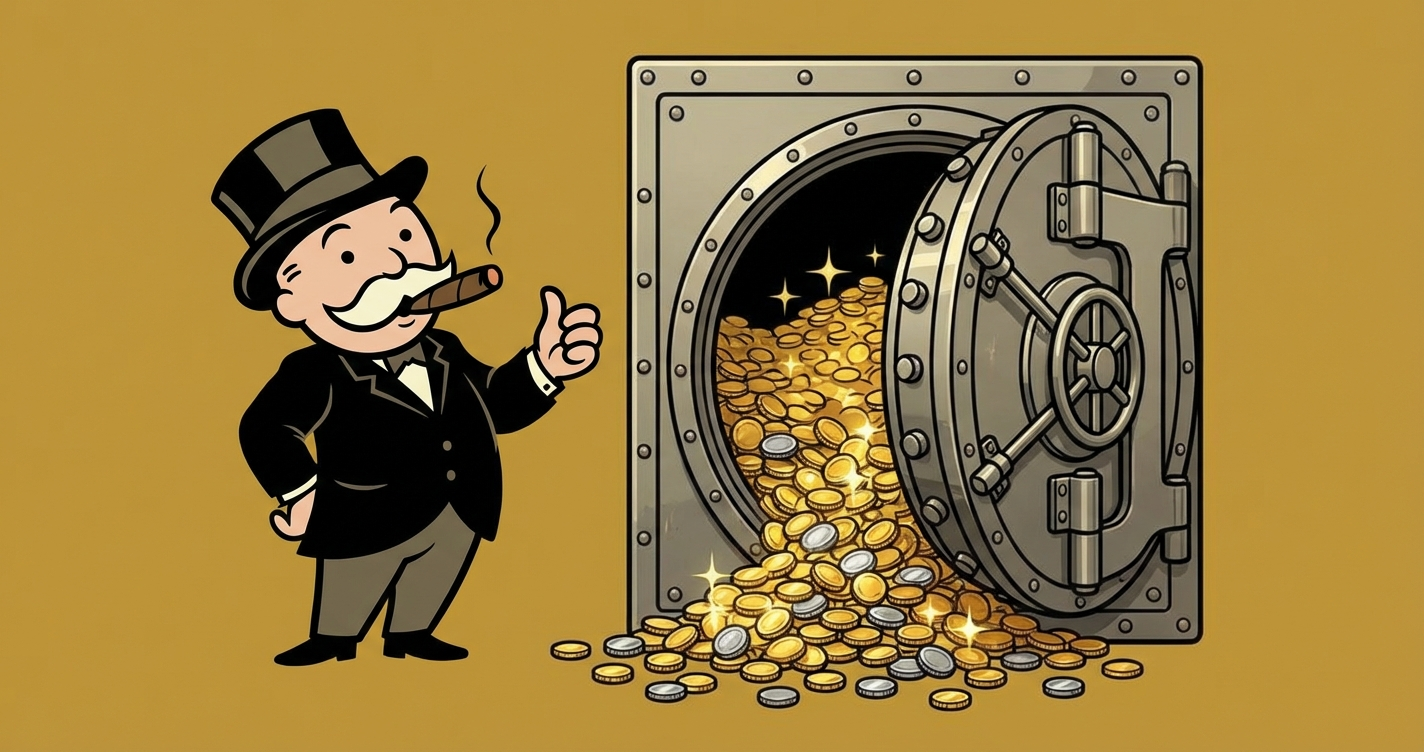
\includegraphics[width=2.5cm]{../../public/images/bonhomme-flipping-coin.jpeg}
\end{center}

Le \textbf{Dirty Man Safe} est la solution que les stackers américains les plus avisés utilisent depuis des années. Le principe~: un tube étanche en PVC renforcé, conçu pour être \textbf{enterré dans le sol de votre jardin}.

Invisible, silencieux, imperméable, résistant à la corrosion --- c'est littéralement un coffre-fort enfoui sous terre. Aucun cambrioleur ne peut le trouver s'il ne sait pas où creuser.

\textbf{Les modèles disponibles~:}

\begin{center}
\begin{tabular}{|l|l|l|l|}
\hline
\rowcolor{gold!20} \textbf{Modèle} & \textbf{Capacité} & \textbf{Dimensions} & \textbf{Pièces 1oz} \\
\hline
Medium & Standard & 3 x 5 pouces & 100 pièces \\
\hline
Large & Grande & 3.5 x 7 pouces & 170 pièces \\
\hline
Extra Large & Maximum & 4 x 10 pouces & 300 pièces \\
\hline
\end{tabular}
\end{center}

\textbf{Comment ça fonctionne~:}
\begin{enumerate}
  \item Choisissez un endroit discret dans votre jardin
  \item Creusez un trou à la profondeur recommandée
  \item Insérez le sleeve (manchon) fourni
  \item Placez vos pièces dans le tube étanche
  \item Refermez hermétiquement avec le Teflon tape inclus
  \item Rebouchez --- votre trésor est invisible
\end{enumerate}

\textbf{Avantages~:}
\begin{itemize}
  \item \textbf{Discrétion absolue} : introuvable sans savoir où chercher
  \item \textbf{Aucun frais récurrent} : achat unique
  \item \textbf{Étanchéité totale} : protège de l'humidité et de la corrosion
  \item \textbf{Pas de risque de contrepartie} : vos pièces sont chez vous
  \item \textbf{Résistance au feu} : sous terre, vos pièces survivront à un incendie
\end{itemize}

\textbf{Précautions~:}
\begin{itemize}
  \item Notez l'emplacement exact et les coordonnées GPS
  \item Informez une personne de confiance ou intégrez l'info dans votre testament
  \item Enveloppez vos pièces dans du papier neutre ou des capsules avant enfouissement
\end{itemize}

Retrouvez le Dirty Man Safe et nos recommandations de stockage sur \href{https://bullionradar.fr/solutions-stockage}{\textbf{BullionRadar.fr}}

\goldsep

\subsection*{Comparatif des solutions de stockage}

\begin{center}
\begin{tabular}{|l|l|l|l|l|}
\hline
\rowcolor{gold!20} \textbf{Solution} & \textbf{Sécurité} & \textbf{Coût} & \textbf{Discrétion} & \textbf{Accès} \\
\hline
Garde dealer & 5/5 & Frais annuels & 3/5 & Différé \\
\hline
Coffre domicile & 4/5 & Achat unique & 3/5 & Immédiat \\
\hline
Dirty Man Safe & 5/5 & Achat unique & 5/5 & Quelques minutes \\
\hline
Banque (coffre) & 3/5 & Frais annuels & 2/5 & Heures ouverture \\
\hline
\end{tabular}
\end{center}

\newpage

% =============================================================================
% RESSOURCES
% =============================================================================
\section*{Ressources pour aller plus loin}
\addcontentsline{toc}{section}{Ressources pour aller plus loin}

\subsection*{Sites de référence}

\href{https://bullionradar.fr}{\textbf{BullionRadar.fr}} --- Comparez les prix de 50+ pièces d'or et d'argent chez les dealers français en temps réel. L'outil indispensable avant chaque achat.

\textbf{LBMA} (London Bullion Market Association) --- L'autorité mondiale de référence pour les cours de l'or et de l'argent. Publie les cours officiels du matin et de l'après-midi (\textit{AM/PM fix}).

\textbf{COMEX} (New York) --- La principale bourse de contrats à terme sur les métaux précieux. Le cours spot mondial est largement déterminé par les échanges sur le COMEX.

\href{https://silverinstitute.org}{\textbf{The Silver Institute}} --- Publie chaque année le \textit{World Silver Survey}, la référence mondiale sur l'offre et la demande d'argent.

\subsection*{Communautés en ligne}

\textbf{Reddit r/Silverbugs} --- La communauté internationale des stackers d'argent. Partage de pièces, retours d'expérience, discussions sur les prix et les dealers.

\textbf{Reddit r/Gold} --- L'équivalent pour l'or. Analyses, questions débutants, photos de stacks.

\textbf{Reddit r/WallStreetSilver} --- Communauté orientée silver squeeze, arguments fondamentaux sur la sous-valorisation de l'argent.

\subsection*{Lectures recommandées}

\begin{itemize}
  \item \textit{The Case for Silver} --- Ted Butler (analyse fondamentale du marché de l'argent)
  \item \textit{Gold: The Once and Future Money} --- Nathan Lewis (histoire monétaire de l'or)
  \item \textit{The ABCs of Gold Investing} --- Michael J. Kosares (guide pratique pour débutants)
\end{itemize}

\subsection*{Indicateurs à surveiller}

\begin{center}
\begin{tabular}{ll}
\toprule
Indicateur & Source \\
\midrule
Cours spot or & \href{https://bullionradar.fr/cours-or}{\textbf{BullionRadar.fr}} \\
Cours spot argent & \href{https://bullionradar.fr/cours-argent}{\textbf{BullionRadar.fr}} \\
Prix dealers (comparatif) & \href{https://bullionradar.fr}{\textbf{BullionRadar.fr}} \\
Ratio or/argent & Macrotrends \\
Stocks COMEX argent & CME Group (cmegroup.com) \\
Achats banques centrales & World Gold Council \\
Demande ETF argent & iShares, WisdomTree \\
World Silver Survey & Silver Institute \\
\bottomrule
\end{tabular}
\end{center}

\subsection*{Dealers français de référence}

\begin{itemize}
  \item \textbf{Godot \& Fils} --- Paris, l'un des plus anciens dealers français
  \item \textbf{Or.fr} --- Achat/vente en ligne, interface moderne
  \item \textbf{Pièces-Or.com} --- Spécialiste pièces françaises et européennes
\end{itemize}

\textit{BullionRadar.fr compare leurs prix en temps réel pour vous garantir le meilleur tarif.}

\newpage

% =============================================================================
% CONCLUSION
% =============================================================================
\section*{Conclusion}
\addcontentsline{toc}{section}{Conclusion}

\begin{center}
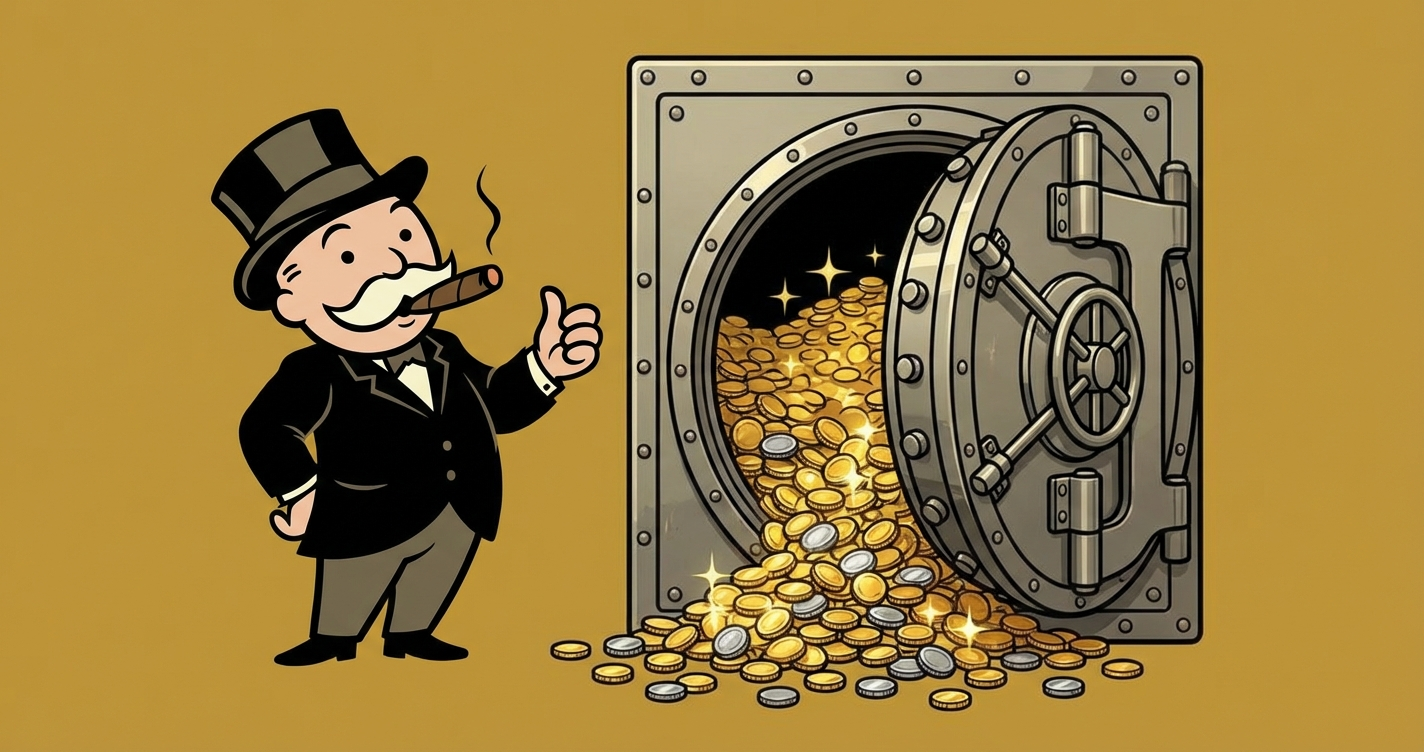
\includegraphics[width=4cm]{../../public/images/bonhomme-coffre-fort.jpeg}
\end{center}

Stacker de l'or et de l'argent c'est \textbf{accessible à tous}. Les règles du bon stacker~:

\begin{enumerate}
  \item \textbf{Commencez petit} --- une pièce à la fois
  \item \textbf{Stackez régulièrement} --- DCA (dollar cost averaging)
  \item \textbf{Comparez toujours} les prix avant d'acheter
  \item \textbf{Pensez long terme} --- l'or protège sur 10, 20, 30 ans
  \item \textbf{Stockez en sécurité} --- coffre personnel ou service de garde
\end{enumerate}

\goldsep

\begin{center}
Rendez-vous sur \href{https://bullionradar.fr}{\textbf{BullionRadar.fr}}\\
pour comparer les prix et les caractéristiques\\
de plus de \textbf{50 pièces d'investissement}.
\end{center}

\goldsep

\begin{center}
\textit{\textcolor{gold!70}{Ce guide est fourni à titre informatif. Il ne constitue pas un conseil en investissement.}}

\href{https://bullionradar.fr}{\textbf{BullionRadar.fr}} --- Le comparateur indépendant de pièces d'or et d'argent en France.
\end{center}

\newpage

% =============================================================================
% GLOSSAIRE
% =============================================================================
\section*{Glossaire du Stacker}
\addcontentsline{toc}{section}{Glossaire du Stacker}

\textbf{Avers} : Face principale d'une pièce, généralement celle qui porte l'effigie du souverain ou un symbole national.

\textbf{Revers} : Dos d'une pièce, portant généralement le motif principal (aigle, feuille d'érable, etc.).

\textbf{Bullion} (ou \textit{bullion coin}) : Pièce d'investissement dont la valeur est principalement déterminée par son contenu en métal précieux, par opposition aux pièces de collection.

\textbf{DCA} (\textit{Dollar Cost Averaging}) : Stratégie d'investissement consistant à acheter régulièrement une quantité fixe de métal, indépendamment du cours.

\textbf{Finesse} (ou pureté) : Proportion de métal précieux dans une pièce, exprimée en millièmes (ex: 999\permil{} = 99,9\% d'argent pur).

\textbf{Métal spot} : Cours international du métal en temps réel, coté sur les marchés à terme (COMEX, LBMA).

\textbf{Once troy} : Unité de masse utilisée pour les métaux précieux. 1 once troy = 31,1035 grammes (différente de l'once ordinaire de 28,35g).

\textbf{Prime} (ou \textit{premium}) : Pourcentage payé au-dessus du cours spot lors de l'achat d'une pièce. Inclut les coûts de frappe, marges du dealer, et rareté éventuelle.

\textbf{Ratio or/argent} : Nombre d'onces d'argent nécessaires pour acheter une once d'or. Indicateur clé de valorisation relative des deux métaux.

\textbf{Round} : Médaille ou disque en métal précieux sans statut de monnaie légale (ex: Buffalo argent). Soumis à TVA 20\% en France.

\textbf{Spot} : Voir \textit{métal spot}. Par extension, «~acheter au spot~» signifie acheter au prix du marché sans prime.

\textbf{Stack} : L'ensemble des métaux précieux physiques détenus par un investisseur. Également utilisé comme verbe («~stacker~» = accumuler).

\textbf{Stacker} : Investisseur qui accumule méthodiquement des pièces d'or et/ou d'argent sur le long terme.

\textbf{TMP} : Taxe sur les Métaux Précieux. En France, taxe forfaitaire de 11,5\% applicable lors de la revente d'or ou d'argent par un particulier, si le régime des plus-values n'est pas choisi.

\textbf{TVA} : Taxe sur la Valeur Ajoutée. En France~: 0\% pour les pièces d'argent avec cours légal actuel, 20\% pour les pièces démonétisées et les rounds.

\textbf{Tube} : Conditionnement standard pour les pièces bullion. Un tube contient généralement 20 ou 25 pièces d'une once (ex: tube de 25 Maple Leaf).

\end{document}
